\documentclass[twoside]{book}

% Packages required by doxygen
\usepackage{fixltx2e}
\usepackage{calc}
\usepackage{doxygen}
\usepackage[export]{adjustbox} % also loads graphicx
\usepackage{graphicx}
\usepackage[utf8]{inputenc}
\usepackage{makeidx}
\usepackage{multicol}
\usepackage{multirow}
\PassOptionsToPackage{warn}{textcomp}
\usepackage{textcomp}
\usepackage[nointegrals]{wasysym}
\usepackage[table]{xcolor}

% Font selection
\usepackage[T1]{fontenc}
\usepackage[scaled=.90]{helvet}
\usepackage{courier}
\usepackage{amssymb}
\usepackage{sectsty}
\renewcommand{\familydefault}{\sfdefault}
\allsectionsfont{%
  \fontseries{bc}\selectfont%
  \color{darkgray}%
}
\renewcommand{\DoxyLabelFont}{%
  \fontseries{bc}\selectfont%
  \color{darkgray}%
}
\newcommand{\+}{\discretionary{\mbox{\scriptsize$\hookleftarrow$}}{}{}}

% Page & text layout
\usepackage{geometry}
\geometry{%
  a4paper,%
  top=2.5cm,%
  bottom=2.5cm,%
  left=2.5cm,%
  right=2.5cm%
}
\tolerance=750
\hfuzz=15pt
\hbadness=750
\setlength{\emergencystretch}{15pt}
\setlength{\parindent}{0cm}
\setlength{\parskip}{3ex plus 2ex minus 2ex}
\makeatletter
\renewcommand{\paragraph}{%
  \@startsection{paragraph}{4}{0ex}{-1.0ex}{1.0ex}{%
    \normalfont\normalsize\bfseries\SS@parafont%
  }%
}
\renewcommand{\subparagraph}{%
  \@startsection{subparagraph}{5}{0ex}{-1.0ex}{1.0ex}{%
    \normalfont\normalsize\bfseries\SS@subparafont%
  }%
}
\makeatother

% Headers & footers
\usepackage{fancyhdr}
\pagestyle{fancyplain}
\fancyhead[LE]{\fancyplain{}{\bfseries\thepage}}
\fancyhead[CE]{\fancyplain{}{}}
\fancyhead[RE]{\fancyplain{}{\bfseries\leftmark}}
\fancyhead[LO]{\fancyplain{}{\bfseries\rightmark}}
\fancyhead[CO]{\fancyplain{}{}}
\fancyhead[RO]{\fancyplain{}{\bfseries\thepage}}
\fancyfoot[LE]{\fancyplain{}{}}
\fancyfoot[CE]{\fancyplain{}{}}
\fancyfoot[RE]{\fancyplain{}{\bfseries\scriptsize Generated by Doxygen }}
\fancyfoot[LO]{\fancyplain{}{\bfseries\scriptsize Generated by Doxygen }}
\fancyfoot[CO]{\fancyplain{}{}}
\fancyfoot[RO]{\fancyplain{}{}}
\renewcommand{\footrulewidth}{0.4pt}
\renewcommand{\chaptermark}[1]{%
  \markboth{#1}{}%
}
\renewcommand{\sectionmark}[1]{%
  \markright{\thesection\ #1}%
}

% Indices & bibliography
\usepackage{natbib}
\usepackage[titles]{tocloft}
\setcounter{tocdepth}{3}
\setcounter{secnumdepth}{5}
\makeindex

% Hyperlinks (required, but should be loaded last)
\usepackage{ifpdf}
\ifpdf
  \usepackage[pdftex,pagebackref=true]{hyperref}
\else
  \usepackage[ps2pdf,pagebackref=true]{hyperref}
\fi
\hypersetup{%
  colorlinks=true,%
  linkcolor=blue,%
  citecolor=blue,%
  unicode%
}

% Custom commands
\newcommand{\clearemptydoublepage}{%
  \newpage{\pagestyle{empty}\cleardoublepage}%
}

\usepackage{caption}
\captionsetup{labelsep=space,justification=centering,font={bf},singlelinecheck=off,skip=4pt,position=top}

%===== C O N T E N T S =====

\begin{document}

% Titlepage & ToC
\hypersetup{pageanchor=false,
             bookmarksnumbered=true,
             pdfencoding=unicode
            }
\pagenumbering{alph}
\begin{titlepage}
\vspace*{7cm}
\begin{center}%
{\Large R\+P\+G2D }\\
\vspace*{1cm}
{\large Generated by Doxygen 1.8.14}\\
\end{center}
\end{titlepage}
\clearemptydoublepage
\pagenumbering{roman}
\tableofcontents
\clearemptydoublepage
\pagenumbering{arabic}
\hypersetup{pageanchor=true}

%--- Begin generated contents ---
\chapter{Namespace Index}
\section{Namespace List}
Here is a list of all documented namespaces with brief descriptions\+:\begin{DoxyCompactList}
\item\contentsline{section}{\mbox{\hyperlink{namespace_r_p_g2_d}{R\+P\+G2D}} }{\pageref{namespace_r_p_g2_d}}{}
\item\contentsline{section}{\mbox{\hyperlink{namespace_r_p_g2_d_1_1_a_p_i}{R\+P\+G2\+D.\+A\+PI}} }{\pageref{namespace_r_p_g2_d_1_1_a_p_i}}{}
\item\contentsline{section}{\mbox{\hyperlink{namespace_r_p_g2_d_1_1_base_classes}{R\+P\+G2\+D.\+Base\+Classes}} }{\pageref{namespace_r_p_g2_d_1_1_base_classes}}{}
\item\contentsline{section}{\mbox{\hyperlink{namespace_r_p_g2_d_1_1_interfaces}{R\+P\+G2\+D.\+Interfaces}} }{\pageref{namespace_r_p_g2_d_1_1_interfaces}}{}
\item\contentsline{section}{\mbox{\hyperlink{namespace_r_p_g2_d_1_1_managers}{R\+P\+G2\+D.\+Managers}} }{\pageref{namespace_r_p_g2_d_1_1_managers}}{}
\item\contentsline{section}{\mbox{\hyperlink{namespace_r_p_g2_d_1_1_registers}{R\+P\+G2\+D.\+Registers}} }{\pageref{namespace_r_p_g2_d_1_1_registers}}{}
\end{DoxyCompactList}

\chapter{Hierarchical Index}
\section{Class Hierarchy}
This inheritance list is sorted roughly, but not completely, alphabetically\+:\begin{DoxyCompactList}
\item \contentsline{section}{R\+P\+G2\+D.\+A\+P\+I.\+Adjusted\+Sprite}{\pageref{class_r_p_g2_d_1_1_a_p_i_1_1_adjusted_sprite}}{}
\item \contentsline{section}{R\+P\+G2\+D.\+Base\+Classes.\+Block}{\pageref{class_r_p_g2_d_1_1_base_classes_1_1_block}}{}
\item \contentsline{section}{R\+P\+G2\+D.\+Registers.\+Block\+Register}{\pageref{class_r_p_g2_d_1_1_registers_1_1_block_register}}{}
\item \contentsline{section}{R\+P\+G2\+D.\+Chunk}{\pageref{class_r_p_g2_d_1_1_chunk}}{}
\item \contentsline{section}{R\+P\+G2\+D.\+Interfaces.\+I\+Game\+Object\+Holder}{\pageref{interface_r_p_g2_d_1_1_interfaces_1_1_i_game_object_holder}}{}
\item \contentsline{section}{R\+P\+G2\+D.\+Base\+Classes.\+Mod}{\pageref{class_r_p_g2_d_1_1_base_classes_1_1_mod}}{}
\item \contentsline{section}{R\+P\+G2\+D.\+Managers.\+Mod\+Manager}{\pageref{class_r_p_g2_d_1_1_managers_1_1_mod_manager}}{}
\item Mono\+Behaviour\begin{DoxyCompactList}
\item \contentsline{section}{R\+P\+G2\+D.\+Game\+Entry}{\pageref{class_r_p_g2_d_1_1_game_entry}}{}
\end{DoxyCompactList}
\item \contentsline{section}{R\+P\+G2\+D.\+Base\+Classes.\+Player}{\pageref{class_r_p_g2_d_1_1_base_classes_1_1_player}}{}
\item \contentsline{section}{R\+P\+G2\+D.\+Registers.\+Player\+Register}{\pageref{class_r_p_g2_d_1_1_registers_1_1_player_register}}{}
\item \contentsline{section}{R\+P\+G2\+D.\+A\+P\+I.\+Random\+Math}{\pageref{class_r_p_g2_d_1_1_a_p_i_1_1_random_math}}{}
\item \contentsline{section}{R\+P\+G2\+D.\+Texture\+Atlas}{\pageref{class_r_p_g2_d_1_1_texture_atlas}}{}
\item \contentsline{section}{R\+P\+G2\+D.\+Managers.\+Texture\+Manager}{\pageref{class_r_p_g2_d_1_1_managers_1_1_texture_manager}}{}
\item \contentsline{section}{R\+P\+G2\+D.\+A\+P\+I.\+World}{\pageref{class_r_p_g2_d_1_1_a_p_i_1_1_world}}{}
\end{DoxyCompactList}

\chapter{Class Index}
\section{Class List}
Here are the classes, structs, unions and interfaces with brief descriptions\+:\begin{DoxyCompactList}
\item\contentsline{section}{\mbox{\hyperlink{class_r_p_g2_d_1_1_a_p_i_1_1_adjusted_sprite}{R\+P\+G2\+D.\+A\+P\+I.\+Adjusted\+Sprite}} }{\pageref{class_r_p_g2_d_1_1_a_p_i_1_1_adjusted_sprite}}{}
\item\contentsline{section}{\mbox{\hyperlink{class_r_p_g2_d_1_1_base_classes_1_1_block}{R\+P\+G2\+D.\+Base\+Classes.\+Block}} }{\pageref{class_r_p_g2_d_1_1_base_classes_1_1_block}}{}
\item\contentsline{section}{\mbox{\hyperlink{class_r_p_g2_d_1_1_registers_1_1_block_register}{R\+P\+G2\+D.\+Registers.\+Block\+Register}} }{\pageref{class_r_p_g2_d_1_1_registers_1_1_block_register}}{}
\item\contentsline{section}{\mbox{\hyperlink{class_r_p_g2_d_1_1_chunk}{R\+P\+G2\+D.\+Chunk}} }{\pageref{class_r_p_g2_d_1_1_chunk}}{}
\item\contentsline{section}{\mbox{\hyperlink{class_r_p_g2_d_1_1_game_entry}{R\+P\+G2\+D.\+Game\+Entry}} }{\pageref{class_r_p_g2_d_1_1_game_entry}}{}
\item\contentsline{section}{\mbox{\hyperlink{interface_r_p_g2_d_1_1_interfaces_1_1_i_game_object_holder}{R\+P\+G2\+D.\+Interfaces.\+I\+Game\+Object\+Holder}} }{\pageref{interface_r_p_g2_d_1_1_interfaces_1_1_i_game_object_holder}}{}
\item\contentsline{section}{\mbox{\hyperlink{class_r_p_g2_d_1_1_base_classes_1_1_mod}{R\+P\+G2\+D.\+Base\+Classes.\+Mod}} }{\pageref{class_r_p_g2_d_1_1_base_classes_1_1_mod}}{}
\item\contentsline{section}{\mbox{\hyperlink{class_r_p_g2_d_1_1_managers_1_1_mod_manager}{R\+P\+G2\+D.\+Managers.\+Mod\+Manager}} }{\pageref{class_r_p_g2_d_1_1_managers_1_1_mod_manager}}{}
\item\contentsline{section}{\mbox{\hyperlink{class_r_p_g2_d_1_1_base_classes_1_1_player}{R\+P\+G2\+D.\+Base\+Classes.\+Player}} }{\pageref{class_r_p_g2_d_1_1_base_classes_1_1_player}}{}
\item\contentsline{section}{\mbox{\hyperlink{class_r_p_g2_d_1_1_registers_1_1_player_register}{R\+P\+G2\+D.\+Registers.\+Player\+Register}} }{\pageref{class_r_p_g2_d_1_1_registers_1_1_player_register}}{}
\item\contentsline{section}{\mbox{\hyperlink{class_r_p_g2_d_1_1_a_p_i_1_1_random_math}{R\+P\+G2\+D.\+A\+P\+I.\+Random\+Math}} }{\pageref{class_r_p_g2_d_1_1_a_p_i_1_1_random_math}}{}
\item\contentsline{section}{\mbox{\hyperlink{class_r_p_g2_d_1_1_texture_atlas}{R\+P\+G2\+D.\+Texture\+Atlas}} }{\pageref{class_r_p_g2_d_1_1_texture_atlas}}{}
\item\contentsline{section}{\mbox{\hyperlink{class_r_p_g2_d_1_1_managers_1_1_texture_manager}{R\+P\+G2\+D.\+Managers.\+Texture\+Manager}} }{\pageref{class_r_p_g2_d_1_1_managers_1_1_texture_manager}}{}
\item\contentsline{section}{\mbox{\hyperlink{class_r_p_g2_d_1_1_a_p_i_1_1_world}{R\+P\+G2\+D.\+A\+P\+I.\+World}} }{\pageref{class_r_p_g2_d_1_1_a_p_i_1_1_world}}{}
\end{DoxyCompactList}

\chapter{Namespace Documentation}
\hypertarget{namespace_r_p_g2_d}{}\section{R\+P\+G2D Namespace Reference}
\label{namespace_r_p_g2_d}\index{R\+P\+G2D@{R\+P\+G2D}}
\subsection*{Namespaces}
\begin{DoxyCompactItemize}
\end{DoxyCompactItemize}
\subsection*{Classes}
\begin{DoxyCompactItemize}
\item 
class \mbox{\hyperlink{class_r_p_g2_d_1_1_chunk}{Chunk}}
\item 
class \mbox{\hyperlink{class_r_p_g2_d_1_1_game_entry}{Game\+Entry}}
\item 
class \mbox{\hyperlink{class_r_p_g2_d_1_1_texture_atlas}{Texture\+Atlas}}
\end{DoxyCompactItemize}

\hypertarget{namespace_r_p_g2_d_1_1_a_p_i}{}\section{R\+P\+G2\+D.\+A\+PI Namespace Reference}
\label{namespace_r_p_g2_d_1_1_a_p_i}\index{R\+P\+G2\+D.\+A\+PI@{R\+P\+G2\+D.\+A\+PI}}
\subsection*{Classes}
\begin{DoxyCompactItemize}
\item 
class \mbox{\hyperlink{class_r_p_g2_d_1_1_a_p_i_1_1_adjusted_sprite}{Adjusted\+Sprite}}
\item 
class \mbox{\hyperlink{class_r_p_g2_d_1_1_a_p_i_1_1_random_math}{Random\+Math}}
\item 
class \mbox{\hyperlink{class_r_p_g2_d_1_1_a_p_i_1_1_world}{World}}
\end{DoxyCompactItemize}

\hypertarget{namespace_r_p_g2_d_1_1_base_classes}{}\section{R\+P\+G2\+D.\+Base\+Classes Namespace Reference}
\label{namespace_r_p_g2_d_1_1_base_classes}\index{R\+P\+G2\+D.\+Base\+Classes@{R\+P\+G2\+D.\+Base\+Classes}}
\subsection*{Classes}
\begin{DoxyCompactItemize}
\item 
class \mbox{\hyperlink{class_r_p_g2_d_1_1_base_classes_1_1_block}{Block}}
\item 
class \mbox{\hyperlink{class_r_p_g2_d_1_1_base_classes_1_1_mod}{Mod}}
\item 
class \mbox{\hyperlink{class_r_p_g2_d_1_1_base_classes_1_1_player}{Player}}
\end{DoxyCompactItemize}

\hypertarget{namespace_r_p_g2_d_1_1_interfaces}{}\section{R\+P\+G2\+D.\+Interfaces Namespace Reference}
\label{namespace_r_p_g2_d_1_1_interfaces}\index{R\+P\+G2\+D.\+Interfaces@{R\+P\+G2\+D.\+Interfaces}}
\subsection*{Classes}
\begin{DoxyCompactItemize}
\item 
interface \mbox{\hyperlink{interface_r_p_g2_d_1_1_interfaces_1_1_i_game_object_holder}{I\+Game\+Object\+Holder}}
\end{DoxyCompactItemize}

\hypertarget{namespace_r_p_g2_d_1_1_managers}{}\section{R\+P\+G2\+D.\+Managers Namespace Reference}
\label{namespace_r_p_g2_d_1_1_managers}\index{R\+P\+G2\+D.\+Managers@{R\+P\+G2\+D.\+Managers}}
\subsection*{Classes}
\begin{DoxyCompactItemize}
\item 
class \mbox{\hyperlink{class_r_p_g2_d_1_1_managers_1_1_mod_manager}{Mod\+Manager}}
\item 
class \mbox{\hyperlink{class_r_p_g2_d_1_1_managers_1_1_texture_manager}{Texture\+Manager}}
\end{DoxyCompactItemize}

\hypertarget{namespace_r_p_g2_d_1_1_registers}{}\section{R\+P\+G2\+D.\+Registers Namespace Reference}
\label{namespace_r_p_g2_d_1_1_registers}\index{R\+P\+G2\+D.\+Registers@{R\+P\+G2\+D.\+Registers}}
\subsection*{Classes}
\begin{DoxyCompactItemize}
\item 
class \mbox{\hyperlink{class_r_p_g2_d_1_1_registers_1_1_block_register}{Block\+Register}}
\item 
class \mbox{\hyperlink{class_r_p_g2_d_1_1_registers_1_1_player_register}{Player\+Register}}
\end{DoxyCompactItemize}

\chapter{Class Documentation}
\hypertarget{class_r_p_g2_d_1_1_a_p_i_1_1_adjusted_sprite}{}\section{R\+P\+G2\+D.\+A\+P\+I.\+Adjusted\+Sprite Class Reference}
\label{class_r_p_g2_d_1_1_a_p_i_1_1_adjusted_sprite}\index{R\+P\+G2\+D.\+A\+P\+I.\+Adjusted\+Sprite@{R\+P\+G2\+D.\+A\+P\+I.\+Adjusted\+Sprite}}
\subsection*{Static Public Member Functions}
\begin{DoxyCompactItemize}
\item 
static Sprite \mbox{\hyperlink{class_r_p_g2_d_1_1_a_p_i_1_1_adjusted_sprite_a4aa452347705855c021fe3ef81689922}{Create}} (Texture2D texture, Rect rect, Vector2 pivot, float ppu)
\begin{DoxyCompactList}\small\item\em Creates a new Adjusted Sprite, the syntax is exactly the same as for the normal Unity\+Engine Sprite. \end{DoxyCompactList}\end{DoxyCompactItemize}


\subsection{Member Function Documentation}
\mbox{\Hypertarget{class_r_p_g2_d_1_1_a_p_i_1_1_adjusted_sprite_a4aa452347705855c021fe3ef81689922}\label{class_r_p_g2_d_1_1_a_p_i_1_1_adjusted_sprite_a4aa452347705855c021fe3ef81689922}} 
\index{R\+P\+G2\+D\+::\+A\+P\+I\+::\+Adjusted\+Sprite@{R\+P\+G2\+D\+::\+A\+P\+I\+::\+Adjusted\+Sprite}!Create@{Create}}
\index{Create@{Create}!R\+P\+G2\+D\+::\+A\+P\+I\+::\+Adjusted\+Sprite@{R\+P\+G2\+D\+::\+A\+P\+I\+::\+Adjusted\+Sprite}}
\subsubsection{\texorpdfstring{Create()}{Create()}}
{\footnotesize\ttfamily static Sprite R\+P\+G2\+D.\+A\+P\+I.\+Adjusted\+Sprite.\+Create (\begin{DoxyParamCaption}\item[{Texture2D}]{texture,  }\item[{Rect}]{rect,  }\item[{Vector2}]{pivot,  }\item[{float}]{ppu }\end{DoxyParamCaption})\hspace{0.3cm}{\ttfamily [inline]}, {\ttfamily [static]}}



Creates a new Adjusted Sprite, the syntax is exactly the same as for the normal Unity\+Engine Sprite. 


\begin{DoxyParams}{Parameters}
{\em texture} & \\
\hline
{\em rect} & \\
\hline
{\em pivot} & \\
\hline
{\em ppu} & \\
\hline
\end{DoxyParams}
\begin{DoxyReturn}{Returns}

\end{DoxyReturn}


The documentation for this class was generated from the following file\+:\begin{DoxyCompactItemize}
\item 
Assets/\+Scripts/\+A\+P\+I/Adjusted\+Sprite.\+cs\end{DoxyCompactItemize}

\hypertarget{class_r_p_g2_d_1_1_base_classes_1_1_block}{}\section{R\+P\+G2\+D.\+Base\+Classes.\+Block Class Reference}
\label{class_r_p_g2_d_1_1_base_classes_1_1_block}\index{R\+P\+G2\+D.\+Base\+Classes.\+Block@{R\+P\+G2\+D.\+Base\+Classes.\+Block}}
\subsection*{Public Member Functions}
\begin{DoxyCompactItemize}
\item 
\mbox{\Hypertarget{class_r_p_g2_d_1_1_base_classes_1_1_block_ac2320c31f8f41be781acfa0f22913c25}\label{class_r_p_g2_d_1_1_base_classes_1_1_block_ac2320c31f8f41be781acfa0f22913c25}} 
abstract bool {\bfseries Init} (Vector2\+Int position)
\item 
\mbox{\Hypertarget{class_r_p_g2_d_1_1_base_classes_1_1_block_aae975d41adf645d7ecc1404304ad8cec}\label{class_r_p_g2_d_1_1_base_classes_1_1_block_aae975d41adf645d7ecc1404304ad8cec}} 
abstract \mbox{\hyperlink{class_r_p_g2_d_1_1_base_classes_1_1_block}{Block}} {\bfseries Copy} ()
\end{DoxyCompactItemize}
\subsection*{Public Attributes}
\begin{DoxyCompactItemize}
\item 
\mbox{\Hypertarget{class_r_p_g2_d_1_1_base_classes_1_1_block_a4e123147e87cce54f821ec79082a637f}\label{class_r_p_g2_d_1_1_base_classes_1_1_block_a4e123147e87cce54f821ec79082a637f}} 
Vector2\+Int {\bfseries position}
\end{DoxyCompactItemize}


The documentation for this class was generated from the following file\+:\begin{DoxyCompactItemize}
\item 
Assets/\+Scripts/\+Base\+Classes/Block.\+cs\end{DoxyCompactItemize}

\hypertarget{class_r_p_g2_d_1_1_registers_1_1_block_register}{}\section{R\+P\+G2\+D.\+Registers.\+Block\+Register Class Reference}
\label{class_r_p_g2_d_1_1_registers_1_1_block_register}\index{R\+P\+G2\+D.\+Registers.\+Block\+Register@{R\+P\+G2\+D.\+Registers.\+Block\+Register}}
\subsection*{Static Public Member Functions}
\begin{DoxyCompactItemize}
\item 
\mbox{\Hypertarget{class_r_p_g2_d_1_1_registers_1_1_block_register_a020af5a6f3796d8a206e788110362bcb}\label{class_r_p_g2_d_1_1_registers_1_1_block_register_a020af5a6f3796d8a206e788110362bcb}} 
static void {\bfseries Register\+Block\+Type} (System.\+Type type, string name)
\item 
\mbox{\Hypertarget{class_r_p_g2_d_1_1_registers_1_1_block_register_a2ff9dc52c823f770544b86bbc860e326}\label{class_r_p_g2_d_1_1_registers_1_1_block_register_a2ff9dc52c823f770544b86bbc860e326}} 
static System.\+Type {\bfseries Get\+Registered\+Block\+Type} (string name)
\item 
\mbox{\Hypertarget{class_r_p_g2_d_1_1_registers_1_1_block_register_acf16a3d65525c7b45cc54318b88f6347}\label{class_r_p_g2_d_1_1_registers_1_1_block_register_acf16a3d65525c7b45cc54318b88f6347}} 
static \mbox{\hyperlink{class_r_p_g2_d_1_1_base_classes_1_1_block}{Block}} {\bfseries Get\+Registered\+Block\+Instance} (string name)
\end{DoxyCompactItemize}
\subsection*{Properties}
\begin{DoxyCompactItemize}
\item 
\mbox{\Hypertarget{class_r_p_g2_d_1_1_registers_1_1_block_register_a1c776fafc46f2711643b754cb2e245b6}\label{class_r_p_g2_d_1_1_registers_1_1_block_register_a1c776fafc46f2711643b754cb2e245b6}} 
static Dictionary$<$ string, Type $>$ {\bfseries Block\+Dictionary}\hspace{0.3cm}{\ttfamily  \mbox{[}get\mbox{]}}
\end{DoxyCompactItemize}


The documentation for this class was generated from the following file\+:\begin{DoxyCompactItemize}
\item 
Assets/\+Scripts/\+Registers/Block\+Register.\+cs\end{DoxyCompactItemize}

\hypertarget{class_r_p_g2_d_1_1_chunk}{}\section{R\+P\+G2\+D.\+Chunk Class Reference}
\label{class_r_p_g2_d_1_1_chunk}\index{R\+P\+G2\+D.\+Chunk@{R\+P\+G2\+D.\+Chunk}}
\subsection*{Public Member Functions}
\begin{DoxyCompactItemize}
\item 
\mbox{\Hypertarget{class_r_p_g2_d_1_1_chunk_ade799c25f41b12c842cdf3fd2e59183b}\label{class_r_p_g2_d_1_1_chunk_ade799c25f41b12c842cdf3fd2e59183b}} 
void {\bfseries Set\+Block\+At} (Vector2\+Int position, \mbox{\hyperlink{class_r_p_g2_d_1_1_base_classes_1_1_block}{Base\+Classes.\+Block}} block)
\item 
\mbox{\Hypertarget{class_r_p_g2_d_1_1_chunk_a252a3f5d169d358d1f179b0909836c47}\label{class_r_p_g2_d_1_1_chunk_a252a3f5d169d358d1f179b0909836c47}} 
\mbox{\hyperlink{class_r_p_g2_d_1_1_base_classes_1_1_block}{Base\+Classes.\+Block}} {\bfseries Get\+Block\+At} (Vector2\+Int position)
\end{DoxyCompactItemize}


The documentation for this class was generated from the following file\+:\begin{DoxyCompactItemize}
\item 
Assets/\+Scripts/Chunk.\+cs\end{DoxyCompactItemize}

\hypertarget{class_r_p_g2_d_1_1_game_entry}{}\section{R\+P\+G2\+D.\+Game\+Entry Class Reference}
\label{class_r_p_g2_d_1_1_game_entry}\index{R\+P\+G2\+D.\+Game\+Entry@{R\+P\+G2\+D.\+Game\+Entry}}
Inheritance diagram for R\+P\+G2\+D.\+Game\+Entry\+:\begin{figure}[H]
\begin{center}
\leavevmode
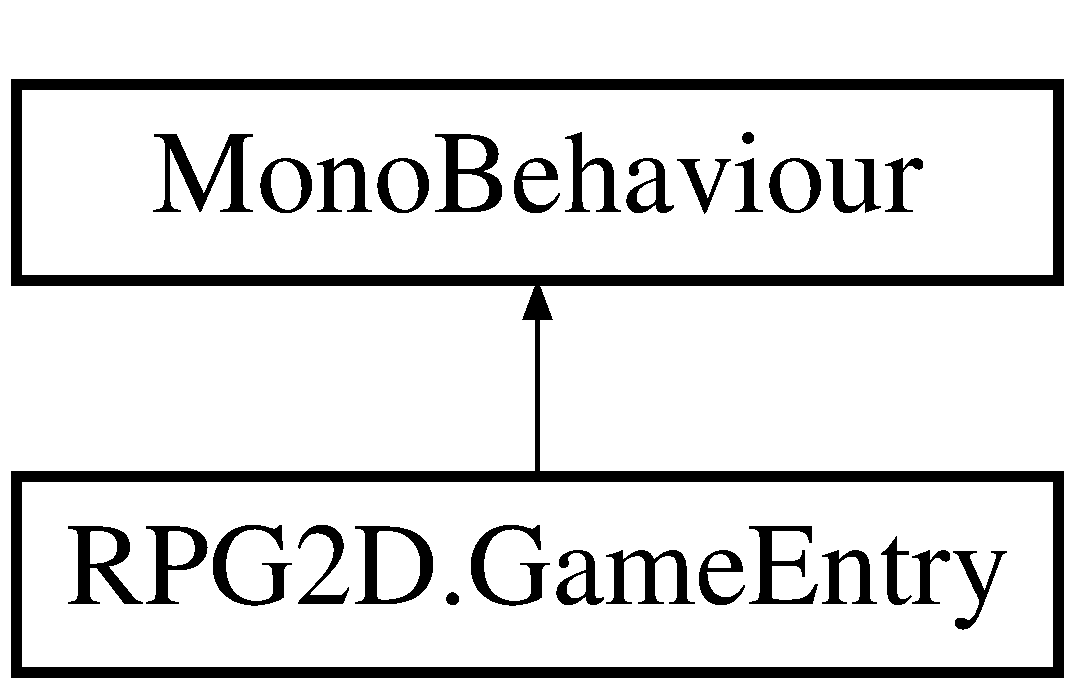
\includegraphics[height=2.000000cm]{class_r_p_g2_d_1_1_game_entry}
\end{center}
\end{figure}


The documentation for this class was generated from the following file\+:\begin{DoxyCompactItemize}
\item 
Assets/\+Scripts/Game\+Entry.\+cs\end{DoxyCompactItemize}

\hypertarget{interface_r_p_g2_d_1_1_interfaces_1_1_i_game_object_holder}{}\section{R\+P\+G2\+D.\+Interfaces.\+I\+Game\+Object\+Holder Interface Reference}
\label{interface_r_p_g2_d_1_1_interfaces_1_1_i_game_object_holder}\index{R\+P\+G2\+D.\+Interfaces.\+I\+Game\+Object\+Holder@{R\+P\+G2\+D.\+Interfaces.\+I\+Game\+Object\+Holder}}
\subsection*{Public Member Functions}
\begin{DoxyCompactItemize}
\item 
\mbox{\Hypertarget{interface_r_p_g2_d_1_1_interfaces_1_1_i_game_object_holder_ab8c3a98986725f8a65db064b60ad3691}\label{interface_r_p_g2_d_1_1_interfaces_1_1_i_game_object_holder_ab8c3a98986725f8a65db064b60ad3691}} 
Game\+Object {\bfseries Return\+Main\+Game\+Object} ()
\item 
\mbox{\Hypertarget{interface_r_p_g2_d_1_1_interfaces_1_1_i_game_object_holder_ac2f4dffda0be3eba1eeac8eb9843b8b4}\label{interface_r_p_g2_d_1_1_interfaces_1_1_i_game_object_holder_ac2f4dffda0be3eba1eeac8eb9843b8b4}} 
List$<$ Game\+Object $>$ {\bfseries Return\+All\+Game\+Objects} ()
\end{DoxyCompactItemize}


The documentation for this interface was generated from the following file\+:\begin{DoxyCompactItemize}
\item 
Assets/\+Scripts/\+Interfaces/I\+Game\+Object\+Holder.\+cs\end{DoxyCompactItemize}

\hypertarget{class_r_p_g2_d_1_1_base_classes_1_1_mod}{}\section{R\+P\+G2\+D.\+Base\+Classes.\+Mod Class Reference}
\label{class_r_p_g2_d_1_1_base_classes_1_1_mod}\index{R\+P\+G2\+D.\+Base\+Classes.\+Mod@{R\+P\+G2\+D.\+Base\+Classes.\+Mod}}
\subsection*{Public Member Functions}
\begin{DoxyCompactItemize}
\item 
\mbox{\Hypertarget{class_r_p_g2_d_1_1_base_classes_1_1_mod_a713fa8c3f8abf773c5dc0c1a73101d9c}\label{class_r_p_g2_d_1_1_base_classes_1_1_mod_a713fa8c3f8abf773c5dc0c1a73101d9c}} 
abstract bool {\bfseries Pre\+Init} ()
\item 
\mbox{\Hypertarget{class_r_p_g2_d_1_1_base_classes_1_1_mod_aa7319cd9bf21558b1fbd8666194eb570}\label{class_r_p_g2_d_1_1_base_classes_1_1_mod_aa7319cd9bf21558b1fbd8666194eb570}} 
abstract bool {\bfseries Init} ()
\item 
\mbox{\Hypertarget{class_r_p_g2_d_1_1_base_classes_1_1_mod_ae1a325679395d1c744c4dbfdffff1dd3}\label{class_r_p_g2_d_1_1_base_classes_1_1_mod_ae1a325679395d1c744c4dbfdffff1dd3}} 
abstract bool {\bfseries Post\+Init} ()
\item 
\mbox{\Hypertarget{class_r_p_g2_d_1_1_base_classes_1_1_mod_a6b9bd6a14be98d51afdc3b3b728ba5ba}\label{class_r_p_g2_d_1_1_base_classes_1_1_mod_a6b9bd6a14be98d51afdc3b3b728ba5ba}} 
abstract bool {\bfseries Load\+Content} ()
\end{DoxyCompactItemize}
\subsection*{Public Attributes}
\begin{DoxyCompactItemize}
\item 
\mbox{\Hypertarget{class_r_p_g2_d_1_1_base_classes_1_1_mod_a973a9ff3e8a8dd20602ae05aefc8ceac}\label{class_r_p_g2_d_1_1_base_classes_1_1_mod_a973a9ff3e8a8dd20602ae05aefc8ceac}} 
string {\bfseries Internal\+Name}
\item 
\mbox{\Hypertarget{class_r_p_g2_d_1_1_base_classes_1_1_mod_aec1779aa5a67f86a3e9671e06c13717a}\label{class_r_p_g2_d_1_1_base_classes_1_1_mod_aec1779aa5a67f86a3e9671e06c13717a}} 
string {\bfseries Visible\+Name}
\item 
\mbox{\Hypertarget{class_r_p_g2_d_1_1_base_classes_1_1_mod_ab92ac6fe5a2edb348dcac666c81e5db5}\label{class_r_p_g2_d_1_1_base_classes_1_1_mod_ab92ac6fe5a2edb348dcac666c81e5db5}} 
string {\bfseries Version}
\end{DoxyCompactItemize}


The documentation for this class was generated from the following file\+:\begin{DoxyCompactItemize}
\item 
Assets/\+Scripts/\+Base\+Classes/Mod.\+cs\end{DoxyCompactItemize}

\hypertarget{class_r_p_g2_d_1_1_managers_1_1_mod_manager}{}\section{R\+P\+G2\+D.\+Managers.\+Mod\+Manager Class Reference}
\label{class_r_p_g2_d_1_1_managers_1_1_mod_manager}\index{R\+P\+G2\+D.\+Managers.\+Mod\+Manager@{R\+P\+G2\+D.\+Managers.\+Mod\+Manager}}
\subsection*{Static Public Member Functions}
\begin{DoxyCompactItemize}
\item 
\mbox{\Hypertarget{class_r_p_g2_d_1_1_managers_1_1_mod_manager_a0535f9c56c324ebf6fefdfe7e0ac55ac}\label{class_r_p_g2_d_1_1_managers_1_1_mod_manager_a0535f9c56c324ebf6fefdfe7e0ac55ac}} 
static bool {\bfseries Load\+Mods} ()
\end{DoxyCompactItemize}


The documentation for this class was generated from the following file\+:\begin{DoxyCompactItemize}
\item 
Assets/\+Scripts/\+Managers/Mod\+Manager.\+cs\end{DoxyCompactItemize}

\hypertarget{class_r_p_g2_d_1_1_base_classes_1_1_player}{}\section{R\+P\+G2\+D.\+Base\+Classes.\+Player Class Reference}
\label{class_r_p_g2_d_1_1_base_classes_1_1_player}\index{R\+P\+G2\+D.\+Base\+Classes.\+Player@{R\+P\+G2\+D.\+Base\+Classes.\+Player}}
\subsection*{Public Member Functions}
\begin{DoxyCompactItemize}
\item 
\mbox{\Hypertarget{class_r_p_g2_d_1_1_base_classes_1_1_player_a0bd1dc7ef5303d8322688335edbd3212}\label{class_r_p_g2_d_1_1_base_classes_1_1_player_a0bd1dc7ef5303d8322688335edbd3212}} 
abstract void {\bfseries Init} ()
\item 
\mbox{\Hypertarget{class_r_p_g2_d_1_1_base_classes_1_1_player_a6334abdf0f7f90b3a4c03f1c379c5fc7}\label{class_r_p_g2_d_1_1_base_classes_1_1_player_a6334abdf0f7f90b3a4c03f1c379c5fc7}} 
abstract void {\bfseries Update} ()
\end{DoxyCompactItemize}


The documentation for this class was generated from the following file\+:\begin{DoxyCompactItemize}
\item 
Assets/\+Scripts/\+Base\+Classes/Player.\+cs\end{DoxyCompactItemize}

\hypertarget{class_r_p_g2_d_1_1_registers_1_1_player_register}{}\section{R\+P\+G2\+D.\+Registers.\+Player\+Register Class Reference}
\label{class_r_p_g2_d_1_1_registers_1_1_player_register}\index{R\+P\+G2\+D.\+Registers.\+Player\+Register@{R\+P\+G2\+D.\+Registers.\+Player\+Register}}
\subsection*{Static Public Member Functions}
\begin{DoxyCompactItemize}
\item 
\mbox{\Hypertarget{class_r_p_g2_d_1_1_registers_1_1_player_register_a0e8f3e6604a4e6ebfa465155fa86b714}\label{class_r_p_g2_d_1_1_registers_1_1_player_register_a0e8f3e6604a4e6ebfa465155fa86b714}} 
static void {\bfseries Instantiate\+Player} ()
\end{DoxyCompactItemize}
\subsection*{Properties}
\begin{DoxyCompactItemize}
\item 
\mbox{\Hypertarget{class_r_p_g2_d_1_1_registers_1_1_player_register_a502741198b14585bb8958f0b7e36724b}\label{class_r_p_g2_d_1_1_registers_1_1_player_register_a502741198b14585bb8958f0b7e36724b}} 
static Type {\bfseries Player\+Type}\hspace{0.3cm}{\ttfamily  \mbox{[}get, set\mbox{]}}
\item 
\mbox{\Hypertarget{class_r_p_g2_d_1_1_registers_1_1_player_register_a08a8fcd89521906380d40e254361a1ac}\label{class_r_p_g2_d_1_1_registers_1_1_player_register_a08a8fcd89521906380d40e254361a1ac}} 
static \mbox{\hyperlink{class_r_p_g2_d_1_1_base_classes_1_1_player}{Base\+Classes.\+Player}} {\bfseries Player}\hspace{0.3cm}{\ttfamily  \mbox{[}get\mbox{]}}
\end{DoxyCompactItemize}


The documentation for this class was generated from the following file\+:\begin{DoxyCompactItemize}
\item 
Assets/\+Scripts/\+Registers/Player\+Register.\+cs\end{DoxyCompactItemize}

\hypertarget{class_r_p_g2_d_1_1_a_p_i_1_1_random_math}{}\section{R\+P\+G2\+D.\+A\+P\+I.\+Random\+Math Class Reference}
\label{class_r_p_g2_d_1_1_a_p_i_1_1_random_math}\index{R\+P\+G2\+D.\+A\+P\+I.\+Random\+Math@{R\+P\+G2\+D.\+A\+P\+I.\+Random\+Math}}
\subsection*{Static Public Member Functions}
\begin{DoxyCompactItemize}
\item 
static int \mbox{\hyperlink{class_r_p_g2_d_1_1_a_p_i_1_1_random_math_a829a5e50051acd046afc856e3ca63981}{Next\+Power\+Of2}} (int n)
\begin{DoxyCompactList}\small\item\em Calculates the next power of two, the power of two is always bigger then n. \end{DoxyCompactList}\end{DoxyCompactItemize}


\subsection{Member Function Documentation}
\mbox{\Hypertarget{class_r_p_g2_d_1_1_a_p_i_1_1_random_math_a829a5e50051acd046afc856e3ca63981}\label{class_r_p_g2_d_1_1_a_p_i_1_1_random_math_a829a5e50051acd046afc856e3ca63981}} 
\index{R\+P\+G2\+D\+::\+A\+P\+I\+::\+Random\+Math@{R\+P\+G2\+D\+::\+A\+P\+I\+::\+Random\+Math}!Next\+Power\+Of2@{Next\+Power\+Of2}}
\index{Next\+Power\+Of2@{Next\+Power\+Of2}!R\+P\+G2\+D\+::\+A\+P\+I\+::\+Random\+Math@{R\+P\+G2\+D\+::\+A\+P\+I\+::\+Random\+Math}}
\subsubsection{\texorpdfstring{Next\+Power\+Of2()}{NextPowerOf2()}}
{\footnotesize\ttfamily static int R\+P\+G2\+D.\+A\+P\+I.\+Random\+Math.\+Next\+Power\+Of2 (\begin{DoxyParamCaption}\item[{int}]{n }\end{DoxyParamCaption})\hspace{0.3cm}{\ttfamily [inline]}, {\ttfamily [static]}}



Calculates the next power of two, the power of two is always bigger then n. 


\begin{DoxyParams}{Parameters}
{\em n} & \\
\hline
\end{DoxyParams}
\begin{DoxyReturn}{Returns}
Next power of two
\end{DoxyReturn}


The documentation for this class was generated from the following file\+:\begin{DoxyCompactItemize}
\item 
Assets/\+Scripts/\+A\+P\+I/Random\+Math.\+cs\end{DoxyCompactItemize}

\hypertarget{class_r_p_g2_d_1_1_texture_atlas}{}\section{R\+P\+G2\+D.\+Texture\+Atlas Class Reference}
\label{class_r_p_g2_d_1_1_texture_atlas}\index{R\+P\+G2\+D.\+Texture\+Atlas@{R\+P\+G2\+D.\+Texture\+Atlas}}
\subsection*{Public Member Functions}
\begin{DoxyCompactItemize}
\item 
void \mbox{\hyperlink{class_r_p_g2_d_1_1_texture_atlas_a6ae525140aaa805c849a86ef345cedfe}{Add\+Texture}} (Texture2D texture, string name)
\begin{DoxyCompactList}\small\item\em Adds a new texture into the atlas, the identifier is the name. \end{DoxyCompactList}\item 
void \mbox{\hyperlink{class_r_p_g2_d_1_1_texture_atlas_a4cec194e23e586d0604379d5bb38fe72}{Add\+Texture}} (string file, string name)
\begin{DoxyCompactList}\small\item\em Adds a new texture into the atlas from file, the identifier is the name. \end{DoxyCompactList}\item 
Rect \mbox{\hyperlink{class_r_p_g2_d_1_1_texture_atlas_a3885f49ace63b00ebcbcfe6a63ca114c}{Get\+Rect}} (string name)
\begin{DoxyCompactList}\small\item\em Gets the rect which is associated with texture name. \end{DoxyCompactList}\item 
void \mbox{\hyperlink{class_r_p_g2_d_1_1_texture_atlas_a1ca0eef601c357e75ffd2e7b7e9348d3}{Pack}} ()
\begin{DoxyCompactList}\small\item\em Packages all textures. \end{DoxyCompactList}\end{DoxyCompactItemize}
\subsection*{Public Attributes}
\begin{DoxyCompactItemize}
\item 
\mbox{\Hypertarget{class_r_p_g2_d_1_1_texture_atlas_a2146b08e7302ca1bfbb4806992ecfc91}\label{class_r_p_g2_d_1_1_texture_atlas_a2146b08e7302ca1bfbb4806992ecfc91}} 
Filter\+Mode {\bfseries Filter\+Mode}
\end{DoxyCompactItemize}
\subsection*{Properties}
\begin{DoxyCompactItemize}
\item 
\mbox{\Hypertarget{class_r_p_g2_d_1_1_texture_atlas_a93e90a6ef0629667c4e726203d7100d5}\label{class_r_p_g2_d_1_1_texture_atlas_a93e90a6ef0629667c4e726203d7100d5}} 
Texture2D {\bfseries Texture}\hspace{0.3cm}{\ttfamily  \mbox{[}get\mbox{]}}
\end{DoxyCompactItemize}


\subsection{Member Function Documentation}
\mbox{\Hypertarget{class_r_p_g2_d_1_1_texture_atlas_a6ae525140aaa805c849a86ef345cedfe}\label{class_r_p_g2_d_1_1_texture_atlas_a6ae525140aaa805c849a86ef345cedfe}} 
\index{R\+P\+G2\+D\+::\+Texture\+Atlas@{R\+P\+G2\+D\+::\+Texture\+Atlas}!Add\+Texture@{Add\+Texture}}
\index{Add\+Texture@{Add\+Texture}!R\+P\+G2\+D\+::\+Texture\+Atlas@{R\+P\+G2\+D\+::\+Texture\+Atlas}}
\subsubsection{\texorpdfstring{Add\+Texture()}{AddTexture()}\hspace{0.1cm}{\footnotesize\ttfamily [1/2]}}
{\footnotesize\ttfamily void R\+P\+G2\+D.\+Texture\+Atlas.\+Add\+Texture (\begin{DoxyParamCaption}\item[{Texture2D}]{texture,  }\item[{string}]{name }\end{DoxyParamCaption})\hspace{0.3cm}{\ttfamily [inline]}}



Adds a new texture into the atlas, the identifier is the name. 


\begin{DoxyParams}{Parameters}
{\em texture} & \\
\hline
{\em name} & \\
\hline
\end{DoxyParams}
\mbox{\Hypertarget{class_r_p_g2_d_1_1_texture_atlas_a4cec194e23e586d0604379d5bb38fe72}\label{class_r_p_g2_d_1_1_texture_atlas_a4cec194e23e586d0604379d5bb38fe72}} 
\index{R\+P\+G2\+D\+::\+Texture\+Atlas@{R\+P\+G2\+D\+::\+Texture\+Atlas}!Add\+Texture@{Add\+Texture}}
\index{Add\+Texture@{Add\+Texture}!R\+P\+G2\+D\+::\+Texture\+Atlas@{R\+P\+G2\+D\+::\+Texture\+Atlas}}
\subsubsection{\texorpdfstring{Add\+Texture()}{AddTexture()}\hspace{0.1cm}{\footnotesize\ttfamily [2/2]}}
{\footnotesize\ttfamily void R\+P\+G2\+D.\+Texture\+Atlas.\+Add\+Texture (\begin{DoxyParamCaption}\item[{string}]{file,  }\item[{string}]{name }\end{DoxyParamCaption})\hspace{0.3cm}{\ttfamily [inline]}}



Adds a new texture into the atlas from file, the identifier is the name. 


\begin{DoxyParams}{Parameters}
{\em file} & \\
\hline
{\em name} & \\
\hline
\end{DoxyParams}
\mbox{\Hypertarget{class_r_p_g2_d_1_1_texture_atlas_a3885f49ace63b00ebcbcfe6a63ca114c}\label{class_r_p_g2_d_1_1_texture_atlas_a3885f49ace63b00ebcbcfe6a63ca114c}} 
\index{R\+P\+G2\+D\+::\+Texture\+Atlas@{R\+P\+G2\+D\+::\+Texture\+Atlas}!Get\+Rect@{Get\+Rect}}
\index{Get\+Rect@{Get\+Rect}!R\+P\+G2\+D\+::\+Texture\+Atlas@{R\+P\+G2\+D\+::\+Texture\+Atlas}}
\subsubsection{\texorpdfstring{Get\+Rect()}{GetRect()}}
{\footnotesize\ttfamily Rect R\+P\+G2\+D.\+Texture\+Atlas.\+Get\+Rect (\begin{DoxyParamCaption}\item[{string}]{name }\end{DoxyParamCaption})\hspace{0.3cm}{\ttfamily [inline]}}



Gets the rect which is associated with texture name. 


\begin{DoxyParams}{Parameters}
{\em name} & \\
\hline
\end{DoxyParams}
\begin{DoxyReturn}{Returns}

\end{DoxyReturn}
\mbox{\Hypertarget{class_r_p_g2_d_1_1_texture_atlas_a1ca0eef601c357e75ffd2e7b7e9348d3}\label{class_r_p_g2_d_1_1_texture_atlas_a1ca0eef601c357e75ffd2e7b7e9348d3}} 
\index{R\+P\+G2\+D\+::\+Texture\+Atlas@{R\+P\+G2\+D\+::\+Texture\+Atlas}!Pack@{Pack}}
\index{Pack@{Pack}!R\+P\+G2\+D\+::\+Texture\+Atlas@{R\+P\+G2\+D\+::\+Texture\+Atlas}}
\subsubsection{\texorpdfstring{Pack()}{Pack()}}
{\footnotesize\ttfamily void R\+P\+G2\+D.\+Texture\+Atlas.\+Pack (\begin{DoxyParamCaption}{ }\end{DoxyParamCaption})\hspace{0.3cm}{\ttfamily [inline]}}



Packages all textures. 



The documentation for this class was generated from the following file\+:\begin{DoxyCompactItemize}
\item 
Assets/\+Scripts/Texture\+Atlas.\+cs\end{DoxyCompactItemize}

\hypertarget{class_r_p_g2_d_1_1_managers_1_1_texture_manager}{}\section{R\+P\+G2\+D.\+Managers.\+Texture\+Manager Class Reference}
\label{class_r_p_g2_d_1_1_managers_1_1_texture_manager}\index{R\+P\+G2\+D.\+Managers.\+Texture\+Manager@{R\+P\+G2\+D.\+Managers.\+Texture\+Manager}}
\subsection*{Static Public Member Functions}
\begin{DoxyCompactItemize}
\item 
\mbox{\Hypertarget{class_r_p_g2_d_1_1_managers_1_1_texture_manager_acb2f5101ac3ee154b8a3f577c4c9594a}\label{class_r_p_g2_d_1_1_managers_1_1_texture_manager_acb2f5101ac3ee154b8a3f577c4c9594a}} 
static \mbox{\hyperlink{class_r_p_g2_d_1_1_texture_atlas}{Texture\+Atlas}} {\bfseries Create\+New\+Texture\+Atlas} (string name)
\item 
\mbox{\Hypertarget{class_r_p_g2_d_1_1_managers_1_1_texture_manager_af0ee0ac25113fa5fc0f2888c1d57eea5}\label{class_r_p_g2_d_1_1_managers_1_1_texture_manager_af0ee0ac25113fa5fc0f2888c1d57eea5}} 
static \mbox{\hyperlink{class_r_p_g2_d_1_1_texture_atlas}{Texture\+Atlas}} {\bfseries Create\+New\+Texture\+Atlas} (string name, \mbox{\hyperlink{class_r_p_g2_d_1_1_texture_atlas}{Texture\+Atlas}} texture\+Atlas)
\item 
\mbox{\Hypertarget{class_r_p_g2_d_1_1_managers_1_1_texture_manager_a1acd65db8c3ffffe820d8145904e7638}\label{class_r_p_g2_d_1_1_managers_1_1_texture_manager_a1acd65db8c3ffffe820d8145904e7638}} 
static void {\bfseries Pack\+All\+Textures} ()
\end{DoxyCompactItemize}
\subsection*{Properties}
\begin{DoxyCompactItemize}
\item 
\mbox{\Hypertarget{class_r_p_g2_d_1_1_managers_1_1_texture_manager_a5364597d24acc20f4020da31ae8bf4a4}\label{class_r_p_g2_d_1_1_managers_1_1_texture_manager_a5364597d24acc20f4020da31ae8bf4a4}} 
static Dictionary$<$ string, \mbox{\hyperlink{class_r_p_g2_d_1_1_texture_atlas}{Texture\+Atlas}} $>$ {\bfseries Texture\+Dictionary}\hspace{0.3cm}{\ttfamily  \mbox{[}get\mbox{]}}
\end{DoxyCompactItemize}


The documentation for this class was generated from the following file\+:\begin{DoxyCompactItemize}
\item 
Assets/\+Scripts/\+Managers/Texture\+Manager.\+cs\end{DoxyCompactItemize}

\hypertarget{class_r_p_g2_d_1_1_a_p_i_1_1_world}{}\section{R\+P\+G2\+D.\+A\+P\+I.\+World Class Reference}
\label{class_r_p_g2_d_1_1_a_p_i_1_1_world}\index{R\+P\+G2\+D.\+A\+P\+I.\+World@{R\+P\+G2\+D.\+A\+P\+I.\+World}}
\subsection*{Static Public Member Functions}
\begin{DoxyCompactItemize}
\item 
static Vector2\+Int \mbox{\hyperlink{class_r_p_g2_d_1_1_a_p_i_1_1_world_ae8afbfcfaaecd14e30cf343404c4336d}{Position\+To\+Chunk}} (Vector2\+Int position)
\begin{DoxyCompactList}\small\item\em Converts \mbox{\hyperlink{class_r_p_g2_d_1_1_a_p_i_1_1_world}{World}} space position to chunk position, so like the chunk number. \end{DoxyCompactList}\item 
static Vector2\+Int \mbox{\hyperlink{class_r_p_g2_d_1_1_a_p_i_1_1_world_a46adadcf2bd6165b14a803f7494c1219}{Position\+To\+Position\+In\+Chunk}} (Vector2\+Int position)
\begin{DoxyCompactList}\small\item\em Converts \mbox{\hyperlink{class_r_p_g2_d_1_1_a_p_i_1_1_world}{World}} space position to the local position inside the chunk. \end{DoxyCompactList}\item 
static void \mbox{\hyperlink{class_r_p_g2_d_1_1_a_p_i_1_1_world_a487e129cc74d77b2e003d197bb50a2a8}{Add\+Chunk}} (Vector2\+Int position)
\begin{DoxyCompactList}\small\item\em Adds a new chunk. \end{DoxyCompactList}\item 
static void \mbox{\hyperlink{class_r_p_g2_d_1_1_a_p_i_1_1_world_a3244e543b87453f50bb93a9d869caa83}{Spawn\+Block}} (Vector2\+Int position, System.\+Type block\+Type)
\begin{DoxyCompactList}\small\item\em Spawns a block at the position. \end{DoxyCompactList}\item 
static void \mbox{\hyperlink{class_r_p_g2_d_1_1_a_p_i_1_1_world_a36e060049f16cc356f30afded645521c}{Spawn\+Block}} (Vector2\+Int position, \mbox{\hyperlink{class_r_p_g2_d_1_1_base_classes_1_1_block}{Base\+Classes.\+Block}} block)
\begin{DoxyCompactList}\small\item\em Spawns a block at the position. (Creates a new instance) \end{DoxyCompactList}\item 
static \mbox{\hyperlink{class_r_p_g2_d_1_1_base_classes_1_1_block}{Base\+Classes.\+Block}} \mbox{\hyperlink{class_r_p_g2_d_1_1_a_p_i_1_1_world_ab5146954658368ff3402fa08f9a556e7}{Get\+Block}} (Vector2\+Int position)
\begin{DoxyCompactList}\small\item\em Gets the block instance at the specified position \end{DoxyCompactList}\item 
static System.\+Type \mbox{\hyperlink{class_r_p_g2_d_1_1_a_p_i_1_1_world_a2e698d1e8265a1040e7713d40aeefb69}{Get\+Block\+Type}} (Vector2\+Int position)
\begin{DoxyCompactList}\small\item\em Gets the block type at the specified position \end{DoxyCompactList}\end{DoxyCompactItemize}


\subsection{Member Function Documentation}
\mbox{\Hypertarget{class_r_p_g2_d_1_1_a_p_i_1_1_world_a487e129cc74d77b2e003d197bb50a2a8}\label{class_r_p_g2_d_1_1_a_p_i_1_1_world_a487e129cc74d77b2e003d197bb50a2a8}} 
\index{R\+P\+G2\+D\+::\+A\+P\+I\+::\+World@{R\+P\+G2\+D\+::\+A\+P\+I\+::\+World}!Add\+Chunk@{Add\+Chunk}}
\index{Add\+Chunk@{Add\+Chunk}!R\+P\+G2\+D\+::\+A\+P\+I\+::\+World@{R\+P\+G2\+D\+::\+A\+P\+I\+::\+World}}
\subsubsection{\texorpdfstring{Add\+Chunk()}{AddChunk()}}
{\footnotesize\ttfamily static void R\+P\+G2\+D.\+A\+P\+I.\+World.\+Add\+Chunk (\begin{DoxyParamCaption}\item[{Vector2\+Int}]{position }\end{DoxyParamCaption})\hspace{0.3cm}{\ttfamily [inline]}, {\ttfamily [static]}}



Adds a new chunk. 


\begin{DoxyParams}{Parameters}
{\em position} & \\
\hline
\end{DoxyParams}
\mbox{\Hypertarget{class_r_p_g2_d_1_1_a_p_i_1_1_world_ab5146954658368ff3402fa08f9a556e7}\label{class_r_p_g2_d_1_1_a_p_i_1_1_world_ab5146954658368ff3402fa08f9a556e7}} 
\index{R\+P\+G2\+D\+::\+A\+P\+I\+::\+World@{R\+P\+G2\+D\+::\+A\+P\+I\+::\+World}!Get\+Block@{Get\+Block}}
\index{Get\+Block@{Get\+Block}!R\+P\+G2\+D\+::\+A\+P\+I\+::\+World@{R\+P\+G2\+D\+::\+A\+P\+I\+::\+World}}
\subsubsection{\texorpdfstring{Get\+Block()}{GetBlock()}}
{\footnotesize\ttfamily static \mbox{\hyperlink{class_r_p_g2_d_1_1_base_classes_1_1_block}{Base\+Classes.\+Block}} R\+P\+G2\+D.\+A\+P\+I.\+World.\+Get\+Block (\begin{DoxyParamCaption}\item[{Vector2\+Int}]{position }\end{DoxyParamCaption})\hspace{0.3cm}{\ttfamily [inline]}, {\ttfamily [static]}}



Gets the block instance at the specified position 


\begin{DoxyParams}{Parameters}
{\em position} & \\
\hline
\end{DoxyParams}
\begin{DoxyReturn}{Returns}
Block instance
\end{DoxyReturn}
\mbox{\Hypertarget{class_r_p_g2_d_1_1_a_p_i_1_1_world_a2e698d1e8265a1040e7713d40aeefb69}\label{class_r_p_g2_d_1_1_a_p_i_1_1_world_a2e698d1e8265a1040e7713d40aeefb69}} 
\index{R\+P\+G2\+D\+::\+A\+P\+I\+::\+World@{R\+P\+G2\+D\+::\+A\+P\+I\+::\+World}!Get\+Block\+Type@{Get\+Block\+Type}}
\index{Get\+Block\+Type@{Get\+Block\+Type}!R\+P\+G2\+D\+::\+A\+P\+I\+::\+World@{R\+P\+G2\+D\+::\+A\+P\+I\+::\+World}}
\subsubsection{\texorpdfstring{Get\+Block\+Type()}{GetBlockType()}}
{\footnotesize\ttfamily static System.\+Type R\+P\+G2\+D.\+A\+P\+I.\+World.\+Get\+Block\+Type (\begin{DoxyParamCaption}\item[{Vector2\+Int}]{position }\end{DoxyParamCaption})\hspace{0.3cm}{\ttfamily [inline]}, {\ttfamily [static]}}



Gets the block type at the specified position 


\begin{DoxyParams}{Parameters}
{\em position} & \\
\hline
\end{DoxyParams}
\begin{DoxyReturn}{Returns}
Block type
\end{DoxyReturn}
\mbox{\Hypertarget{class_r_p_g2_d_1_1_a_p_i_1_1_world_ae8afbfcfaaecd14e30cf343404c4336d}\label{class_r_p_g2_d_1_1_a_p_i_1_1_world_ae8afbfcfaaecd14e30cf343404c4336d}} 
\index{R\+P\+G2\+D\+::\+A\+P\+I\+::\+World@{R\+P\+G2\+D\+::\+A\+P\+I\+::\+World}!Position\+To\+Chunk@{Position\+To\+Chunk}}
\index{Position\+To\+Chunk@{Position\+To\+Chunk}!R\+P\+G2\+D\+::\+A\+P\+I\+::\+World@{R\+P\+G2\+D\+::\+A\+P\+I\+::\+World}}
\subsubsection{\texorpdfstring{Position\+To\+Chunk()}{PositionToChunk()}}
{\footnotesize\ttfamily static Vector2\+Int R\+P\+G2\+D.\+A\+P\+I.\+World.\+Position\+To\+Chunk (\begin{DoxyParamCaption}\item[{Vector2\+Int}]{position }\end{DoxyParamCaption})\hspace{0.3cm}{\ttfamily [inline]}, {\ttfamily [static]}}



Converts \mbox{\hyperlink{class_r_p_g2_d_1_1_a_p_i_1_1_world}{World}} space position to chunk position, so like the chunk number. 


\begin{DoxyParams}{Parameters}
{\em position} & \\
\hline
\end{DoxyParams}
\begin{DoxyReturn}{Returns}
Returns the chunk position.
\end{DoxyReturn}
\mbox{\Hypertarget{class_r_p_g2_d_1_1_a_p_i_1_1_world_a46adadcf2bd6165b14a803f7494c1219}\label{class_r_p_g2_d_1_1_a_p_i_1_1_world_a46adadcf2bd6165b14a803f7494c1219}} 
\index{R\+P\+G2\+D\+::\+A\+P\+I\+::\+World@{R\+P\+G2\+D\+::\+A\+P\+I\+::\+World}!Position\+To\+Position\+In\+Chunk@{Position\+To\+Position\+In\+Chunk}}
\index{Position\+To\+Position\+In\+Chunk@{Position\+To\+Position\+In\+Chunk}!R\+P\+G2\+D\+::\+A\+P\+I\+::\+World@{R\+P\+G2\+D\+::\+A\+P\+I\+::\+World}}
\subsubsection{\texorpdfstring{Position\+To\+Position\+In\+Chunk()}{PositionToPositionInChunk()}}
{\footnotesize\ttfamily static Vector2\+Int R\+P\+G2\+D.\+A\+P\+I.\+World.\+Position\+To\+Position\+In\+Chunk (\begin{DoxyParamCaption}\item[{Vector2\+Int}]{position }\end{DoxyParamCaption})\hspace{0.3cm}{\ttfamily [inline]}, {\ttfamily [static]}}



Converts \mbox{\hyperlink{class_r_p_g2_d_1_1_a_p_i_1_1_world}{World}} space position to the local position inside the chunk. 


\begin{DoxyParams}{Parameters}
{\em position} & \\
\hline
\end{DoxyParams}
\begin{DoxyReturn}{Returns}
Position inside the chunk.
\end{DoxyReturn}
\mbox{\Hypertarget{class_r_p_g2_d_1_1_a_p_i_1_1_world_a3244e543b87453f50bb93a9d869caa83}\label{class_r_p_g2_d_1_1_a_p_i_1_1_world_a3244e543b87453f50bb93a9d869caa83}} 
\index{R\+P\+G2\+D\+::\+A\+P\+I\+::\+World@{R\+P\+G2\+D\+::\+A\+P\+I\+::\+World}!Spawn\+Block@{Spawn\+Block}}
\index{Spawn\+Block@{Spawn\+Block}!R\+P\+G2\+D\+::\+A\+P\+I\+::\+World@{R\+P\+G2\+D\+::\+A\+P\+I\+::\+World}}
\subsubsection{\texorpdfstring{Spawn\+Block()}{SpawnBlock()}\hspace{0.1cm}{\footnotesize\ttfamily [1/2]}}
{\footnotesize\ttfamily static void R\+P\+G2\+D.\+A\+P\+I.\+World.\+Spawn\+Block (\begin{DoxyParamCaption}\item[{Vector2\+Int}]{position,  }\item[{System.\+Type}]{block\+Type }\end{DoxyParamCaption})\hspace{0.3cm}{\ttfamily [inline]}, {\ttfamily [static]}}



Spawns a block at the position. 


\begin{DoxyParams}{Parameters}
{\em position} & \\
\hline
{\em block\+Type} & \\
\hline
\end{DoxyParams}
\mbox{\Hypertarget{class_r_p_g2_d_1_1_a_p_i_1_1_world_a36e060049f16cc356f30afded645521c}\label{class_r_p_g2_d_1_1_a_p_i_1_1_world_a36e060049f16cc356f30afded645521c}} 
\index{R\+P\+G2\+D\+::\+A\+P\+I\+::\+World@{R\+P\+G2\+D\+::\+A\+P\+I\+::\+World}!Spawn\+Block@{Spawn\+Block}}
\index{Spawn\+Block@{Spawn\+Block}!R\+P\+G2\+D\+::\+A\+P\+I\+::\+World@{R\+P\+G2\+D\+::\+A\+P\+I\+::\+World}}
\subsubsection{\texorpdfstring{Spawn\+Block()}{SpawnBlock()}\hspace{0.1cm}{\footnotesize\ttfamily [2/2]}}
{\footnotesize\ttfamily static void R\+P\+G2\+D.\+A\+P\+I.\+World.\+Spawn\+Block (\begin{DoxyParamCaption}\item[{Vector2\+Int}]{position,  }\item[{\mbox{\hyperlink{class_r_p_g2_d_1_1_base_classes_1_1_block}{Base\+Classes.\+Block}}}]{block }\end{DoxyParamCaption})\hspace{0.3cm}{\ttfamily [inline]}, {\ttfamily [static]}}



Spawns a block at the position. (Creates a new instance) 


\begin{DoxyParams}{Parameters}
{\em position} & \\
\hline
{\em block} & \\
\hline
\end{DoxyParams}


The documentation for this class was generated from the following file\+:\begin{DoxyCompactItemize}
\item 
Assets/\+Scripts/\+A\+P\+I/World.\+cs\end{DoxyCompactItemize}

%--- End generated contents ---

% Index
\backmatter
\newpage
\phantomsection
\clearemptydoublepage
\addcontentsline{toc}{chapter}{Index}
\printindex

\end{document}
